\section{Algoritmo GRASP}

\subsection{Introducción}
La idea de este algoritmo es ejecutar una serie de veces nuestro algoritmo GREEDY randomizado y mejorarlo con la búsqueda local, guardando la mejor solución hasta el momento.
Esa randomización se debe a que el método por el cuál dicho algoritmo goloso elige siempre el mejor valor bajo su criterio, es ahora aleatorizada seleccionando al azar entre los primeros k elementos de la
lista de nodos a ser considerado dominante.\\
Para ello, agregamos en el algoritmo Greedy que reciba por parámetro dicho k, de forma tal que al momento de elegir el próximo nodo, en vez de elegir el primero de los nodos ordenados por la cantidad de adyacentes
sin dominar, ahora elige la posición i, que será el número obtenido pseudo-aleatoriamente a través de la función random entre 0 y k. En caso de que este k sea mayor a la cantidad de nodos considerados en la lista, 
k se definirá como la longitud de dicha lista.\\
Un tema importante de GRASP es que nunca termina, y neceista una condición de parada arbitraria. Elegimos, al igual que en LocalSearch, una iteración que busque hasta k veces asumiendo que
de las k*$|$MinConjDominante$|$ posibles soluciones que me puede devolver en cada iteración el algoritmo greedy.

\subsection{Pseudocódigo}

\begin{codebox}
\Procname{$\proc{MCDGrasp}$ (\textbf{in} $Grafo$, \textbf{in} $k$)}{ConjDominante}{Conj}
\li	mejorSolucion = TodosLosVertices
\li \textbf{Para} i=0 hasta k \Do
\li 	instanciaSolucionGreedyRandomized = MCDGreedy(grafo,k)
\li	nuevaSolucion = MCDLocalSearch(instanciaSolucionGreedyRandomized)
\li 	\textbf{Si} cantNodosDominantes(nuevaSolucion) $<$ cantNodosDominantes(mejorSolucion)  \Do
\li		mejorSolucion = nuevaSolucion
	\End
    \End	
\li	\textbf{return} mejorSolucion	
\end{codebox}
Se debe aclarar que tanto LocalSearch como Greedy devuelven ConjuntosDominantes verdaderos, por lo que lo único que importa es la cantidad de nodos devuelta.\\

A continuación se agrega el cambio hecho en el algoritmo greedy para aleatorizar la selección de nodos:\\
\begin{codebox}
\Procname{$\proc{elegirVertice}$ (\textbf{in} $ListaVerticesORdenada$, \textbf{in} $k$)}{proxVertice}{Vertice}	
\li     \textbf{Si} k $>$ $|$ListaVerticesORdenada$|$ \Do
\li 		k = $|$ListaVerticesORdenada$|$;
\li 	posiciónAElegir = random(0,k);
\li	proxVertice = ListaVerticesORdenada[posiciónAElegir]
\li 	\textbf{return} proxVertice
\end{codebox}

\subsection{Análisis de Complejidad}
Por la demostración de la complejidad de la búsqueda local, sabemos que la complejidad es: O($n^2$);\\
Por la demostración de la complejidad del goloso, sabemos que la complejidad es: O($n^3$);\\
Dentro del GRASP se realizan k iteraciones de las siguientes operaciones:
\begin{itemize}
\item Ejecutar algoritmo goloso con random
\item Ejecutar algoritmo localSearch a partir de la solución del goloso
\item Comparar mejorSolución con nuevaSolución (esta operación es en O(1) ya que tanto conseguir el tamaño de un ArrayList en Java como la comparación de enteros es en O(1)) 
\end{itemize}
Esto es O(k*(goloso + localSearch)), que resulta polinomial.\\
Entonces la complejidad resulta O(k*$n^3$);

\subsection{Peor Caso}
Antes de hacer el gráfico, deberíamos calcular cual es el peor caso para este algoritmo. Sin embargo, el mismo depende de dos cosas:
\begin{itemize}
\item La solución random generada por el algoritmo goloso cuando se usa el valor de k. 	Esto es importante, ya que mientras esa solución sea generada de forma pseudo-random, menor cantidad
	de operaciones va a haber en la búsqueda local.
\item No se pudo determinar un peor caso para la búqueda local. Es decir, no se encontró una entrada, en donde la
	cantidad de operaciones que se hagan sean máximas.
\end{itemize}

\subsection{Tests y análisis}
Al igual que en la búsqueda local, en este algoritmo tambien se incremente la cantidad de operaciones a medida
que se incrementa la cantidad de conjuntos dominantes devuelto por la solución greedy.\\
Cabe recordar que en cada iteración, el algoritmo greedy retorna una solución de las k*$|$conjuntoDomniante$|$ posibles soluciones, que después se buscará localmente una mejora en caso de existir a través del camino elegido.\\
Ahora se presenta un algoritmo con un mismo grafo corrido n veces con k random cada vez

\begin{center}
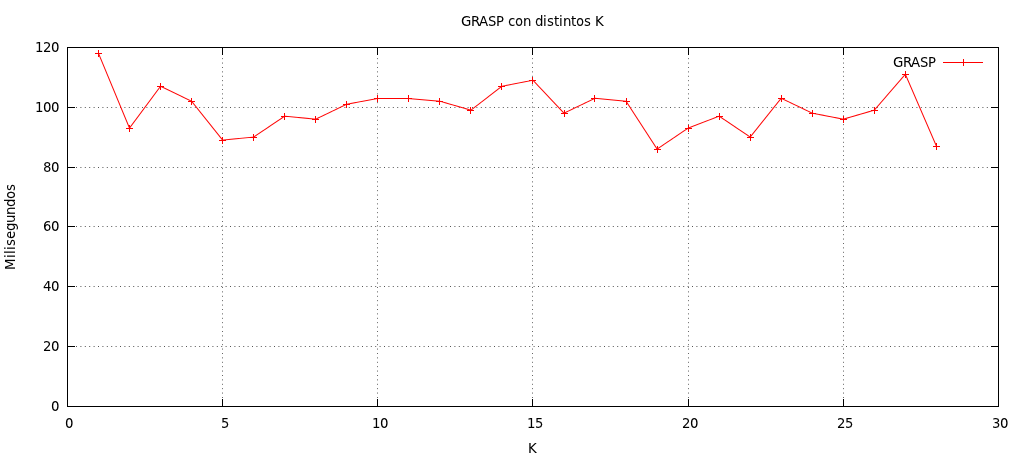
\includegraphics[width=15cm]{./graficos/GRASP_distintosK.png}
\end{center}

Como se puede notar en la imágen, el tiempo no varía ya que k se comporta como una constante al ser siempre menos a la cantidad de nodos, por lo que en caso de saber valores de la entrada en los que sabemos
que Greedy se comportaría mal al elegir siempre el mejor a partir de su estrategia, elegir un k más grande para poder elegir entre más nodos aleatoriamente, no arruina el tiempo de procesamiento.

Ahora se presenta un algoritmo con distintos grafos corrido cada uno con k = 5,10,15,20

\begin{center}
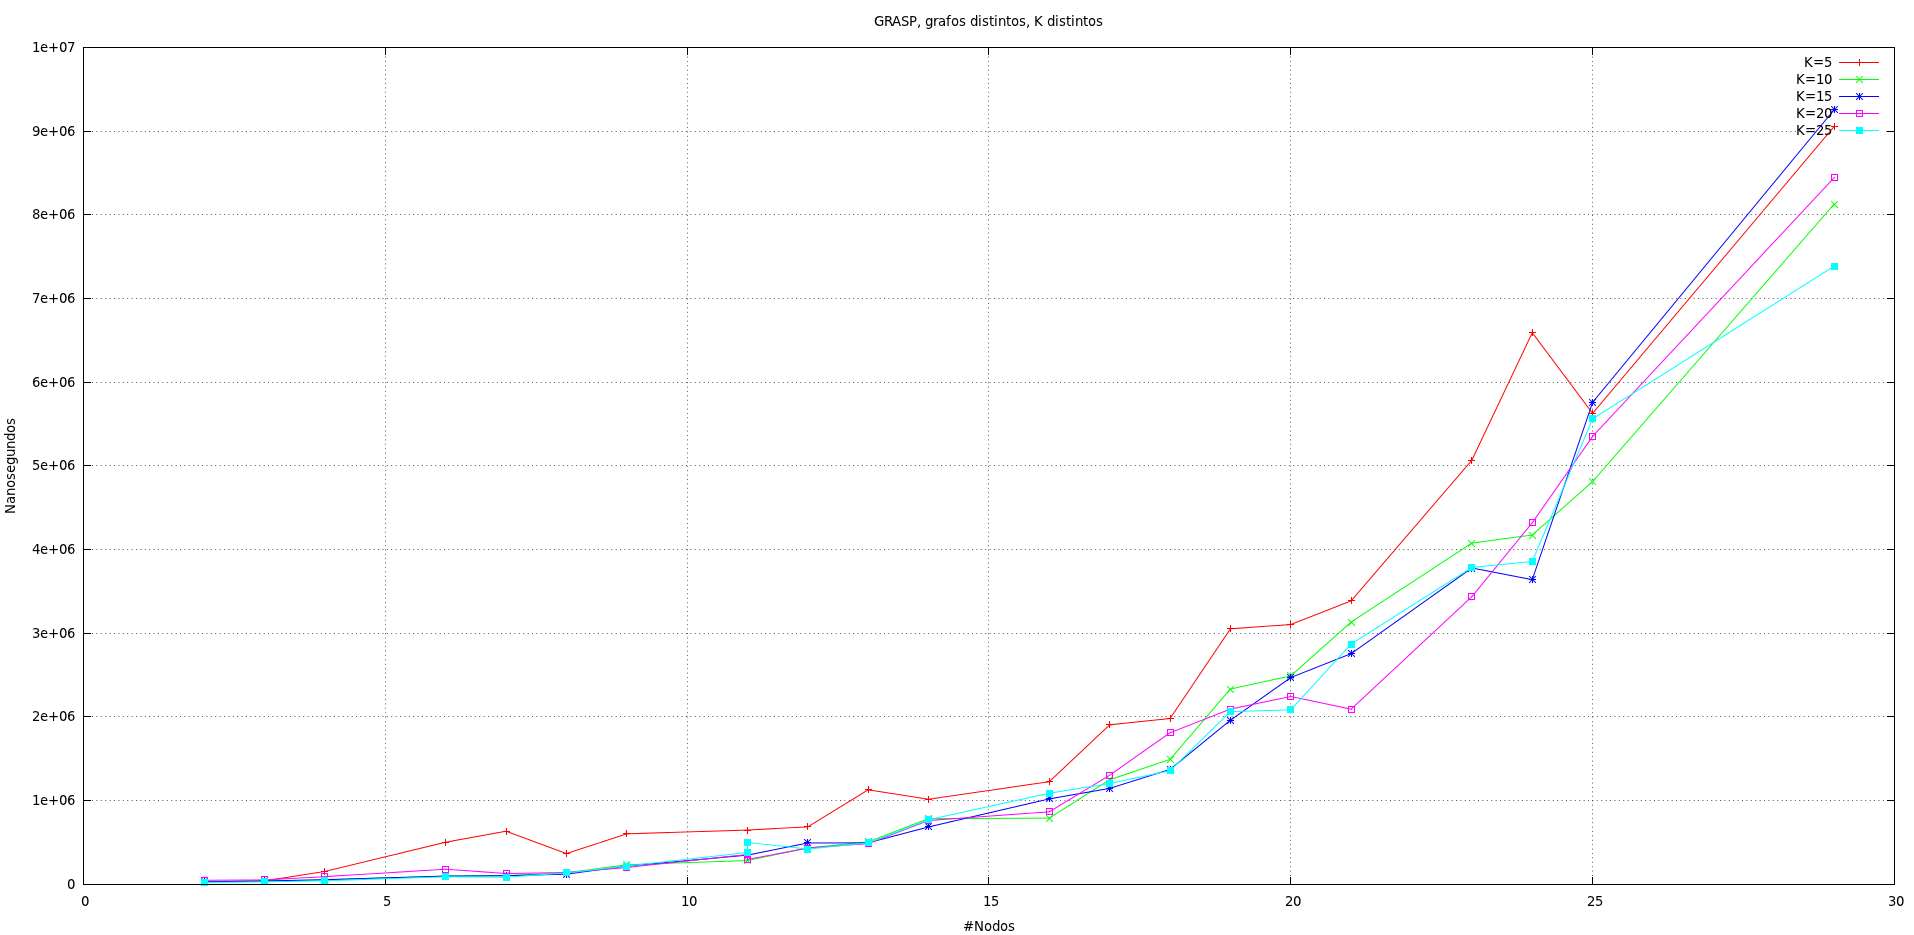
\includegraphics[width=15cm]{./graficos/GRASP_distGrafos_distK.png}
\end{center}

Tal como era esperado el algorimto hace menos operaciones cuando tiene menos nodos y el k multiplica el tiempo como una constante.
Sin embargo, es necesario tener en cuenta que, al depender de otros algoritmos como ser: Greedy y LocalSearch, que tienen una condición de corte distinta a la de este algoritmo, puede pasar que terminen antes o tarden más.
Es así que se explican la falta de paralelismo exacto de los gráficos. Por ejemplo, en caso de que greedy con un k, elija en tres iteraciones un conjunto dominante minimal y sin embargo para otro k elija en más iteraciones.
